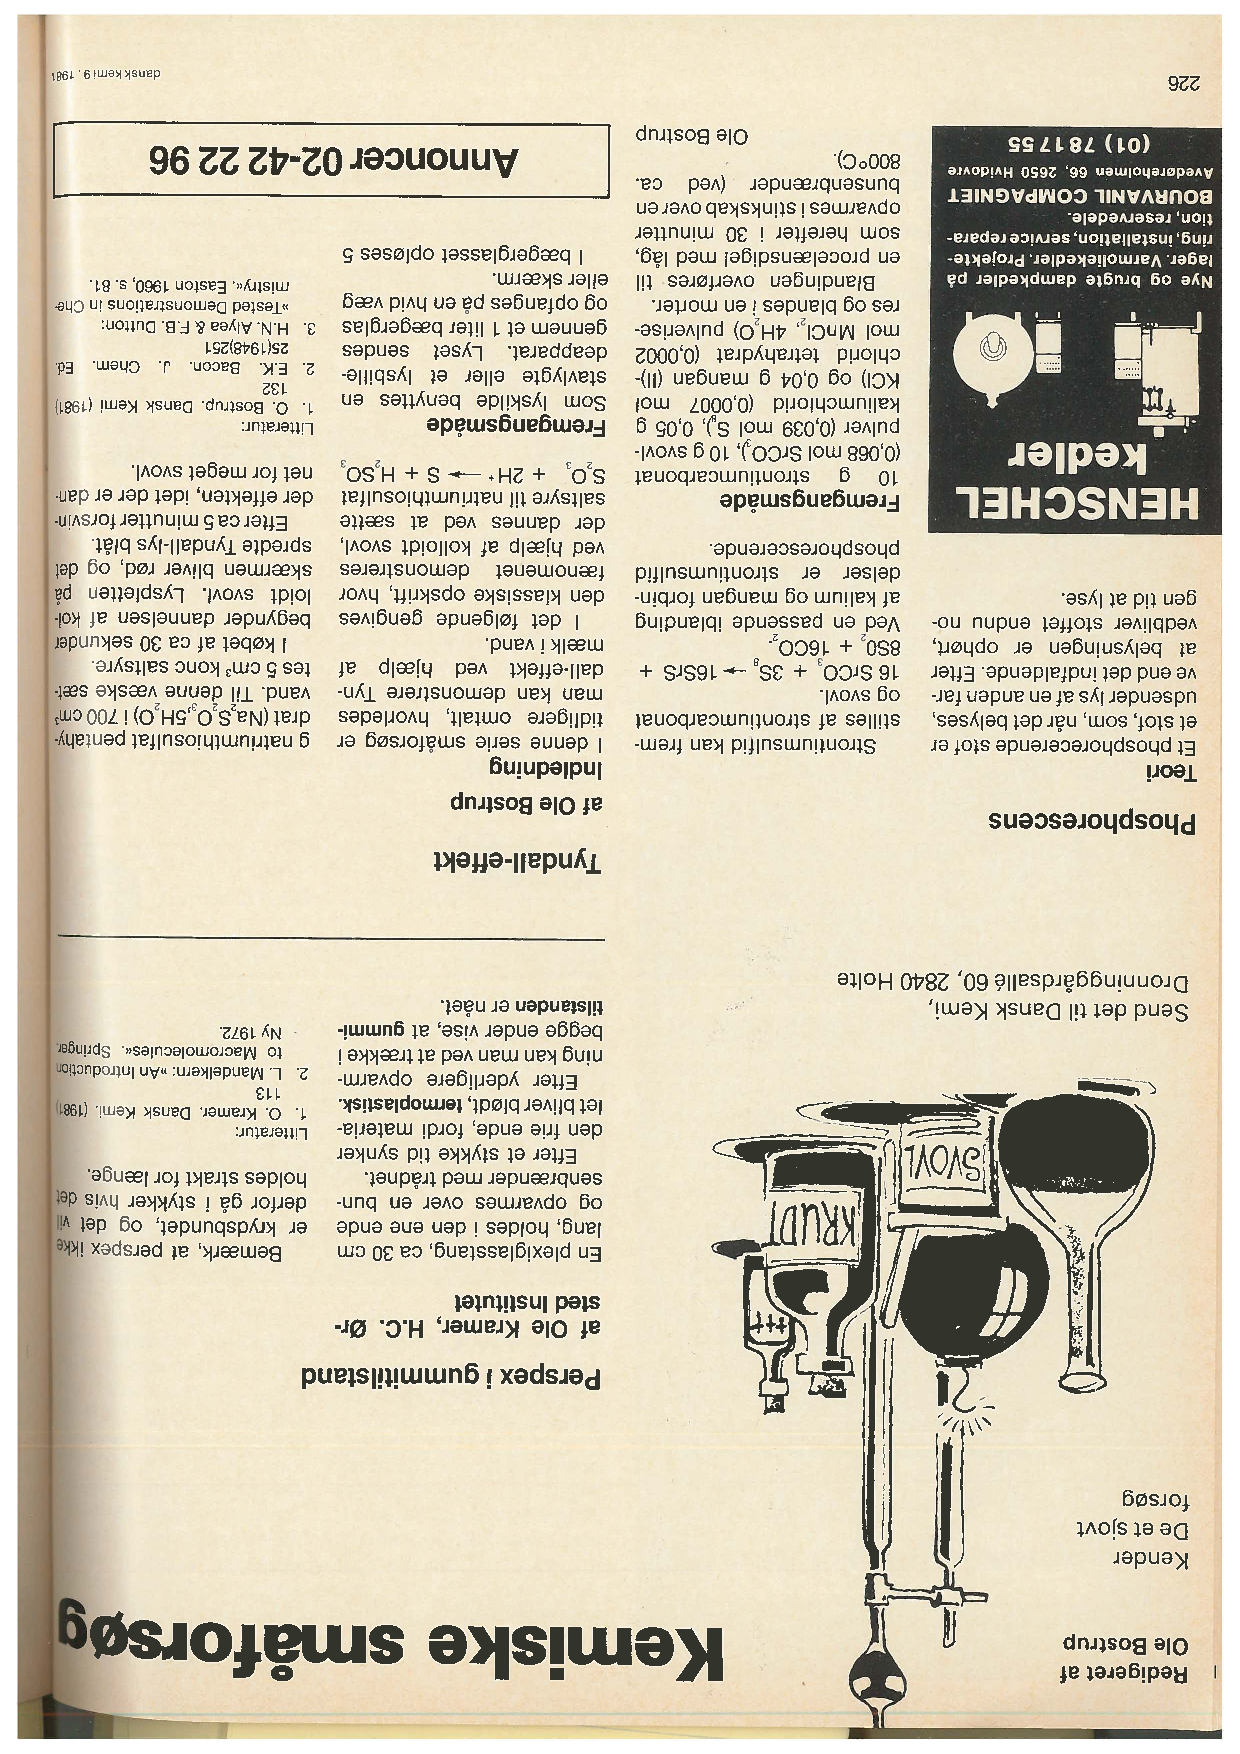
\includepdf[pages=-]{pdfs/1981-62-9-226.pdf}

\emne{Phosphorescens}
\danskkemi{1981-62-9-226}
\forfatter{Ole Bostrup}


\deloverskrift{Teori}

Et phosphorecerende stof er et stof, som, når det
belyses, udsender lys af en anden farve end det
indfaldende. Efter at belysningen er ophørt,
vedbliver stoffet endnu nogen tid at lyse.

Strontiumsulfid kan fremstilles af strontiumcarbonat
og svovl.
\begin{center}
\ch{16 SrCO3 + 2 S8 -> 16 SrS + 8 SO2 + 16 CO2}
\end{center}
Ved en passende iblanding af kalium og mangan
forbindelser er strontiumsulfid phosphorescerende.

\deloverskrift{Fremgangsmåde}

10 g strontiumcarbonat (0,068 mol \ch{SrCO3}), 10 g
svovlpulver (0,039 mol \ch{S8}), 0,05 g kaliumchlorid
(0.0007 mol KCl) og 0,4 g mangan (II)- chlorid
tetrahydrat (0,0002 mol \ch{MnCl2}, \ch{4 H2O}) pulveriseres
og blandes i en morter.
Blandingen overføres til en porcelænsdigel med
låg, som herefter i 30 minutter opvarmes i
stinkskab over en bunsenbrænder (ved ca. 800
gradtegn C).
